\documentclass[a4paper]{article}

\usepackage{amsmath}
\usepackage{amssymb}
\usepackage[margin=1.5cm,
            includefoot,
            footskip=30pt]{geometry}
\usepackage{layout}
\usepackage{graphicx}
\usepackage{subcaption}

\usepackage{biblatex}
\usepackage{pdfpages}
\usepackage{booktabs}

\bibliography{main.bib}
\newcommand{\SSe}{\text{SS}_{\text{error}}}

\title{Suspicion: Recognising and evaluating the effectiveness
       of extortion in the Iterated Prisoner's Dilemma}
\author{Vincent A. Knight \and
        Nikoleta E. Glynatsi \and
        Jonathan Gillard \and
        Marc Harper}
\date{\today}



\begin{document}

\maketitle

\begin{abstract}
    The Iterated Prisoner's Dilemma is a model for rational and evolutionary
    interactive behaviour, having applications in biology, the study of human
    social behaviour, and many other domains.  It is often used to understand
    when and how a rational individual might accept an immediate cost to their
    own utility for the direct benefit of another.

    Much attention has been given to a class of strategies called
    Zero Determinant strategies. It has been theoretically shown that these
    strategies can ``extort'' large classes of other strategies.

    In this work, we describe an approach to identify if observed strategies are
    playing in an extortionate manner. This corresponds to a mathematical model
    of suspicion. Furthermore, experimental analysis of a large tournament with
    204strategies is
    considered. In this setting the most highly performing strategies do not
    play in an extortionate manner against each other but do against lower
    performing strategies.  This suggests that whilst the theory of Zero
    Determinant strategies suggests that memory is not of fundamental importance
    to the evolution of cooperative behaviour, this narrative is incomplete.

    By considering evolutionary frameworks, we use this measure of extortion to
    obtain a statistically significant correlation between the variability of
    behaviour and evolutionary stability. This shows that complex strategies
    that are able to adapt their behaviour for each interaction are more likely 
    to survive the evolutionary process.
\end{abstract}

\section{Introduction}\label{sec:introduction}

Agent-based game-theoretic models have become a stalwart of the underpinning
mathematics of interactive behaviours. One of the major pieces of work in this
area is the pair of computer tournaments run by Robert
Axelrod~\cite{Axelrod1980, Axelrod1980a}. These tournaments pitted submitted
computer strategies against each other in plays of the Iterated Prisoner's
Dilemma, which is a common game where agents can choose to pay a slight cost to
their immediate utility in the hope of building a reputation. This has been used
in economic and evolutionary game theory to understand the evolution of
cooperative behaviour.

In~\cite{Press2012} a class of strategies that can provably extort given
opponents was described. These so called Zero-Determinant (ZD) strategies caused
a substantial reaction in the game theoretic community. As stated
in~\cite{hilbe2015partners}, the American Mathematical Society's news section
stated that `the world of game theory is currently on fire'.
In~\cite{adami2013evolutionary, Hilbe2013, hilbe2013adaptive, hilbe2015partners,
ichinose2018zero, Moran1707} some questions have already been asked about the
true effectiveness of these strategies in an evolutionary setting. For
example~\cite{adami2013evolutionary} showed that ZD strategies were not
evolutionarily stable. Furthermore, in that work it was also postulated that
`evolutionarily successful ZD strategies can be designed that use longer memory
to distinguish self from non-self'.

The main question being asked in this work is: is it possible to recognise this
extortionate ZD behaviour? A mathematical procedure for suspicion is presented,
reflecting the way that the continued actions of an extortionate individual
might raise suspicion.

ZD strategies are defined by a constrained set of transition probabilities
\(p\in\mathbb{R}^4\) (so called memory-one strategies). In this work, a
procedure is offered that will quantify if any strategy is acting in an
extortionate way. A \(p\in\mathbb{R}^4\) can be measured from actual
interactions, regardless of whether or not the strategy is defined in such a
way. In Section~\ref{sec:sserror-zd-strategies} a measure is used
to capture how close a given \(p\in\mathbb{R}^4\) is to being ZD.
This allows for the
recognition of extortionate behaviour even in the cases of numeric inexactitude
that would otherwise imply a strategy was not extortionate. It is also possible
to recognise sophisticated strategies that act extortionately against some
opponents but not others. This was the concept suggested
in~\cite{adami2013evolutionary} when speaking about being able to distinguish
self from non-self.

This work makes use of the Axelrod Python library~\cite{Knight2016, Knight2018}
which contains a large number of Prisoner Dilemma strategies available for
extensive numerical examples.  The approach is presented in
Section~\ref{sec:sserror-zd-strategies}.  All of the code and data discussed in
Section~\ref{sec:numerical-experiments} is open sourced, archived and written
according to best scientific principles~\cite{Wilson2014}. The data archive can
be found at~\cite{vincent_knight_2018_1297075}.  In
Section~\ref{sec:evolutionary-dynamics}, this large tournament is complemented
with an evolutionary consideration that offers some insight in to the
effectiveness of extortionate strategies.

\section{Recognising Extortion}\label{sec:sserror-zd-strategies}

Zero Determinant (ZD) strategies are introduced in~\cite{Press2012} in the
context of matches between two memory-one strategies. Memory-one strategies are
represented as elements of \(\mathbb{R}^4\) mapping a state of \({\{C, D\}}^2\)
to a probability of cooperating. A match between two such strategies creates a
Markov chain with transient states \({\{C, D\}}^2\). The main result
of~\cite{Press2012} is that given two memory-one players \(p,
q\in\mathbb{R}^4\), a linear relationship between the players' scores can be
forced by one of the players.

Using the notation of~\cite{Press2012}, the utilities for player \(p\)
are given by \(S_x=(R, S, T, P)\) and for player \(q\) by \(S_y=(R, T, S, P)\)
and the stationary scores of each player are given by \(S_X\) and \(S_Y\)
respectively. The main result of~\cite{Press2012} is that if

\begin{equation}\label{eqn:linear_relationship_for_p}
    \tilde p=\alpha S_x + \beta S_y + \gamma
\end{equation}

or

\begin{equation}\label{eqn:linear_relationship_for_q}
    \tilde q=\alpha S_x + \beta S_y + \gamma
\end{equation}

where \(\tilde p = (1 - p_1, 1 - p_2, p_3, p_4)\) and
\(\tilde q = (1 - q_1, 1 - q_2, q_3, q_4)\) then:

\begin{equation}
    \alpha S_X + \beta S_Y + \gamma = 0
\end{equation}

In~\cite{Press2012} a particular type of ZD strategy is defined: extortionate
strategies. If:

\begin{equation}\label{eqn:constraint_for_extortion}
    \gamma = - P(\alpha + \beta)
\end{equation}

then the player can ensure they get a score \(\chi\) times
larger than the opponent. This extortion coefficient is given by:

\begin{equation}\label{eqn:definition_of_chi}
    \chi=\frac{-\beta}{\alpha}
\end{equation}

Thus, if (\ref{eqn:constraint_for_extortion}) holds and \(\chi >1\) a player is
said to extort their opponent.
Here, the reverse problem is considered: given a
\(p\in\mathbb{R}^4\) how does one identify \(\alpha, \beta\) if they
exist and is the strategy in fact acting in an extortionate way?

In this case constraints (\ref{eqn:linear_relationship_for_p}) and
(\ref{eqn:constraint_for_extortion}) correspond to:

\begin{align}
    \tilde p_1 & = \alpha R + \beta R - P (\alpha + \beta)
            \label{eqn:condition_for_tilde_p1}\\
    \tilde p_2 & = \alpha S + \beta T - P (\alpha + \beta)
            \label{eqn:condition_for_tilde_p2}\\
    \tilde p_3 & = \alpha T + \beta S - P (\alpha + \beta)
            \label{eqn:condition_for_tilde_p3}\\
    \tilde p_4 & = \alpha P + \beta P - P (\alpha + \beta) = 0
            \label{eqn:condition_for_tilde_p4}
\end{align}

Equation (\ref{eqn:condition_for_tilde_p4}) ensures that \(p_4=\tilde p_4=0\).
Equations (\ref{eqn:condition_for_tilde_p1}-\ref{eqn:condition_for_tilde_p3})
can be used to eliminate \(\alpha, \beta\), giving:

\begin{equation}\label{eqn:planar_definition_of_extortion}
    \tilde p_1 = \frac{(R - P)(\tilde p_2 + \tilde p_3)}{S + T - 2P}
\end{equation}

with:

\begin{equation}\label{eqn:definition_of_chi}
    \chi = \frac{\tilde p_2 (P - T) + \tilde p_3 (S - P)}
                {\tilde p_2 (P - S) + \tilde p_3 (T - P)}
\end{equation}

Given a strategy \(p\in\mathbb{R}^{4}\) equations
(\ref{eqn:condition_for_tilde_p4}-\ref{eqn:definition_of_chi}) can be used to
check if a strategy is extortionate. The conditions correspond to:

\begin{align}
    p_1 & = \frac{(R-P)(p_2 + p_3) - R + T + S - P}{S + T - 2P}
     \label{eqn:condition_for_p1}\\
    p_4 & = 0 \label{eqn:condition_for_p4}\\
    1 & > p_2 + p_3\label{eqn:condition_for_chi}
\end{align}

The algebraic steps necessary to prove these results are available in the
supporting materials, and note that an equivalent formulation was obtained
in~\cite{adami2013evolutionary}.

All extortionate strategies reside on a triangular (\ref{eqn:condition_for_chi})
plane (\ref{eqn:condition_for_p1}) in 3 dimensions (\ref{eqn:condition_for_p4}).
Using this formulation it can be seen that a necessary (but not sufficient)
condition for an extortionate strategy is that it cooperates on average less
than 50\% of the time when in a state of disagreement with the opponent
(\ref{eqn:condition_for_chi}).

As an example, consider the known extortionate strategy \(p=(8 / 9, 1 / 2, 1 /
3, 0)\) from~\cite{Stewart2012} which is referred to as \texttt{Extort-2}. In
this case, for the standard values of \((R, S, T, P) = (3, 0, 5, 1)\)
constraint (\ref{eqn:condition_for_p1}) corresponds to:

\begin{equation}
    p_1 = \frac{2(p_2 + p_3) + 1}{3}
        = \frac{2(1 / 2 + 1 / 3) + 1}{3}
        = \frac{8}{9}
\end{equation}

It is clear that in this case all constraints hold. As a counterexample,
consider the strategy that cooperates 25\% of the time: \(p=(1 /4, 1 / 4, 1 / 4,
1 / 4)\) obeys~(\ref{eqn:condition_for_chi}) but is not extortionate as:

\begin{equation}
    p_1 \ne \frac{2(p_2 + p_3) + 1}{3}
        = \frac{2(1 / 4 + 1 / 4) + 1}{3}
        = \frac{2}{3}
\end{equation}

Not all strategies are memory-one strategies but it is possible to
measure a given \(p\) from any set of interactions between two strategies.
This approach can then be used to confirm that a given strategy is acting
in an extortionate manner even if it is not a memory-one strategy. However, in
practice, if an exact form for \(p\) is not known but measured from observed
plays of the game then measurement and/or numerical error might lead to an
extortionate strategy not being confirmed as such.

As an example consider Table~\ref{tab:actual_plays_of_ZDextort-2} which shows
some actual plays of \(p=(8 / 9, 1 / 2, 1 / 3, 0)\) against an alternating
strategy (\(p=(0, 0, 1, 1)\)):

\begin{table}[!hbtp]
    \begin{tabular}{lllllllllllllllllllll}
\toprule
Turn               &  1 &  2 &  3 &  4 &  5 &  6 &  7 &  8 &  9 &  10 &  11 &  12 &  13 &  14 &  15 &  16 &  17 &  18 &  19 &  20 \\\midrule
(8/9, 1/2, 1/3, 0) &  C &  C &  D &  D &  D &  C &  D &  D &  D &   D &   D &   C &   C &   C &   D &   D &   D &   C &   D &   D \\
Alternator         &  C &  D &  C &  D &  C &  D &  C &  D &  C &   D &   C &   D &   C &   D &   C &   D &   C &   D &   C &   D \\
\bottomrule
\end{tabular}

    \caption{A seeded play of 20 turns of two strategies.}
    \label{tab:actual_plays_of_ZDextort-2}
\end{table}

In this particular instance the measured value of \(p\) for the known
extortionate strategy would be: \((2/2, 1/5, 3/8, 4/4)\) which is does not fit
the definition of a ZD strategy.

Note that measurement of behaviour might in some cases lead to missing values.
For example the strategy \(p=(8 / 9, 1 / 2, 1 / 3, 0)\) when playing against a
cooperator will in fact never visit any state which would allow to measure
\(p_3\) and \(p_4\). To overcome this, it is proposed that if \(s\) is a state
that is not visited than \(p_s\) is approximated using a sensible prior. In
Section~\ref{sec:numerical-experiments} the overall cooperation rate is used.
Another approach to overcoming this measurement error would be to measure our
strategies in a minimalistically noisy environment.

Identifying if a strategy is ZD strategy can be written in the following linear
algebraic form where \(x=(\alpha, \beta)\) and \(p^*=(\tilde p_1 - 1, \tilde p_2
- 1, \tilde p_3, \tilde p_4)\):

\begin{equation}\label{eqn:linear_algebraic_equation_for_p}
    Cx= p^*
\end{equation}

\(C\) corresponds to equations
(\ref{eqn:condition_for_tilde_p1}-\ref{eqn:condition_for_tilde_p3}) and is
given by:

\begin{equation}\label{eqn:definition_of_C}
    C =
    \begin{bmatrix}
        R - P & R- P \\
        S - P & T- P \\
        T - P & S- P \\
        0     & 0 \\
    \end{bmatrix}
\end{equation}

Note that in general, equation (\ref{eqn:linear_algebraic_equation_for_p}) will
not necessarily have a solution. From the Rouch\'{e}-Capelli theorem if there is
a solution it is unique as \(\text{rank}(C)=2\) which is the dimension of the
variable \(x\). The best fitting \(x^*\) is defined by:

\begin{equation}\label{eqn:x_star}
    x^* = \text{argmin}_{x\in\mathbb{R}^2}\|C x- p^*\|_2^2
\end{equation}

Known results~\cite{kutner2004applied, rao1973linear, wakefield2013bayesian} can
now be applied:

\begin{equation}\label{eqn:x_star_formula}
    x^* = {\left(C^{T}C\right)}^{-1}C^{T}p^{*}
\end{equation}

This \(x^*\) corresponds to the nearest ZD strategy to the
measured \(p\). It is in fact a normal projection of \(p\) on to the plane
defined by (\ref{eqn:condition_for_p1}).

The squared norm of the remaining error is referred to as
\(\SSe\):

\begin{equation}\label{eqn:r_squared}
    \SSe = \|C x^*- p^*\|_2^2
\end{equation}

This gives expressions for \(\alpha, \beta\) as \(\alpha=x^*_1\) and
\(\beta=x^*_2\) thus the conditions for a strategy to be acting extortionately
becomes:

\begin{equation}
    -x^*_2 < x^*_1 \label{eqn:measured_condition_for_chi}
\end{equation}

A further known result~~\cite{kutner2004applied, rao1973linear,
wakefield2013bayesian} gives an expression for
\(\SSe\):

\begin{equation}\label{eqn:x_SSError_formula}
    \SSe = {p ^ *} ^ T p ^ * -
           p ^ * C \left(C ^ T C \right) ^ {-1} C ^ T p ^ *
         = {p ^ *} ^ T p ^ * - p ^ * C x ^ *
\end{equation}

Using this approach, the memory-one representation \(p\in\mathbb{R}^4\) of any
strategy against any other can can be measured and if
(\ref{eqn:measured_condition_for_chi}) holds then (\ref{eqn:x_SSError_formula})
can be used to identify if a strategy is acting extortionately.

For a measured \(p\), \(\SSe\) corresponds to the best
fitting \(\alpha, \beta\). Suspicion of
extortion then corresponds to a threshold on the following value
\(\SSe\).

Comparing theoretic and actual plays of the
IPD is not novel, see for example~\cite{Rand2013}.

In the next section, this idea will be illustrated by observing the interactions
that take place in a large computer based tournament of the IPD\@.

\section{Numerical experiments}\label{sec:numerical-experiments}

In~\cite{Stewart2012} results from a tournament with
19 strategies,
were presented with specific consideration given to ZD strategies. This
tournament is reproduced here using the Axelrod-Python
library~\cite{Knight2016}. To obtain a good measure of the corresponding
transition rates for each strategy all matches have been run for
2000turns and every match has been
repeated 60times. All of this
interaction data is available at~\cite{vincent_knight_2018_1297075}. Note that
in the interest of open scientific practice,~\cite{vincent_knight_2018_1297075}
also contains interaction data for noisy and probabilistic ending interactions
which are not investigated here.

Figure~\ref{fig:sserror_in_stewart_plotkin} shows the
\(\SSe\) values for all the strategies in the tournament, as
reported in~\cite{Stewart2012} the extortionate strategy (which has an expected
\(\kappa\) approximately 0) gains a large number of wins.

\begin{figure}[!htbp]
    \centering
    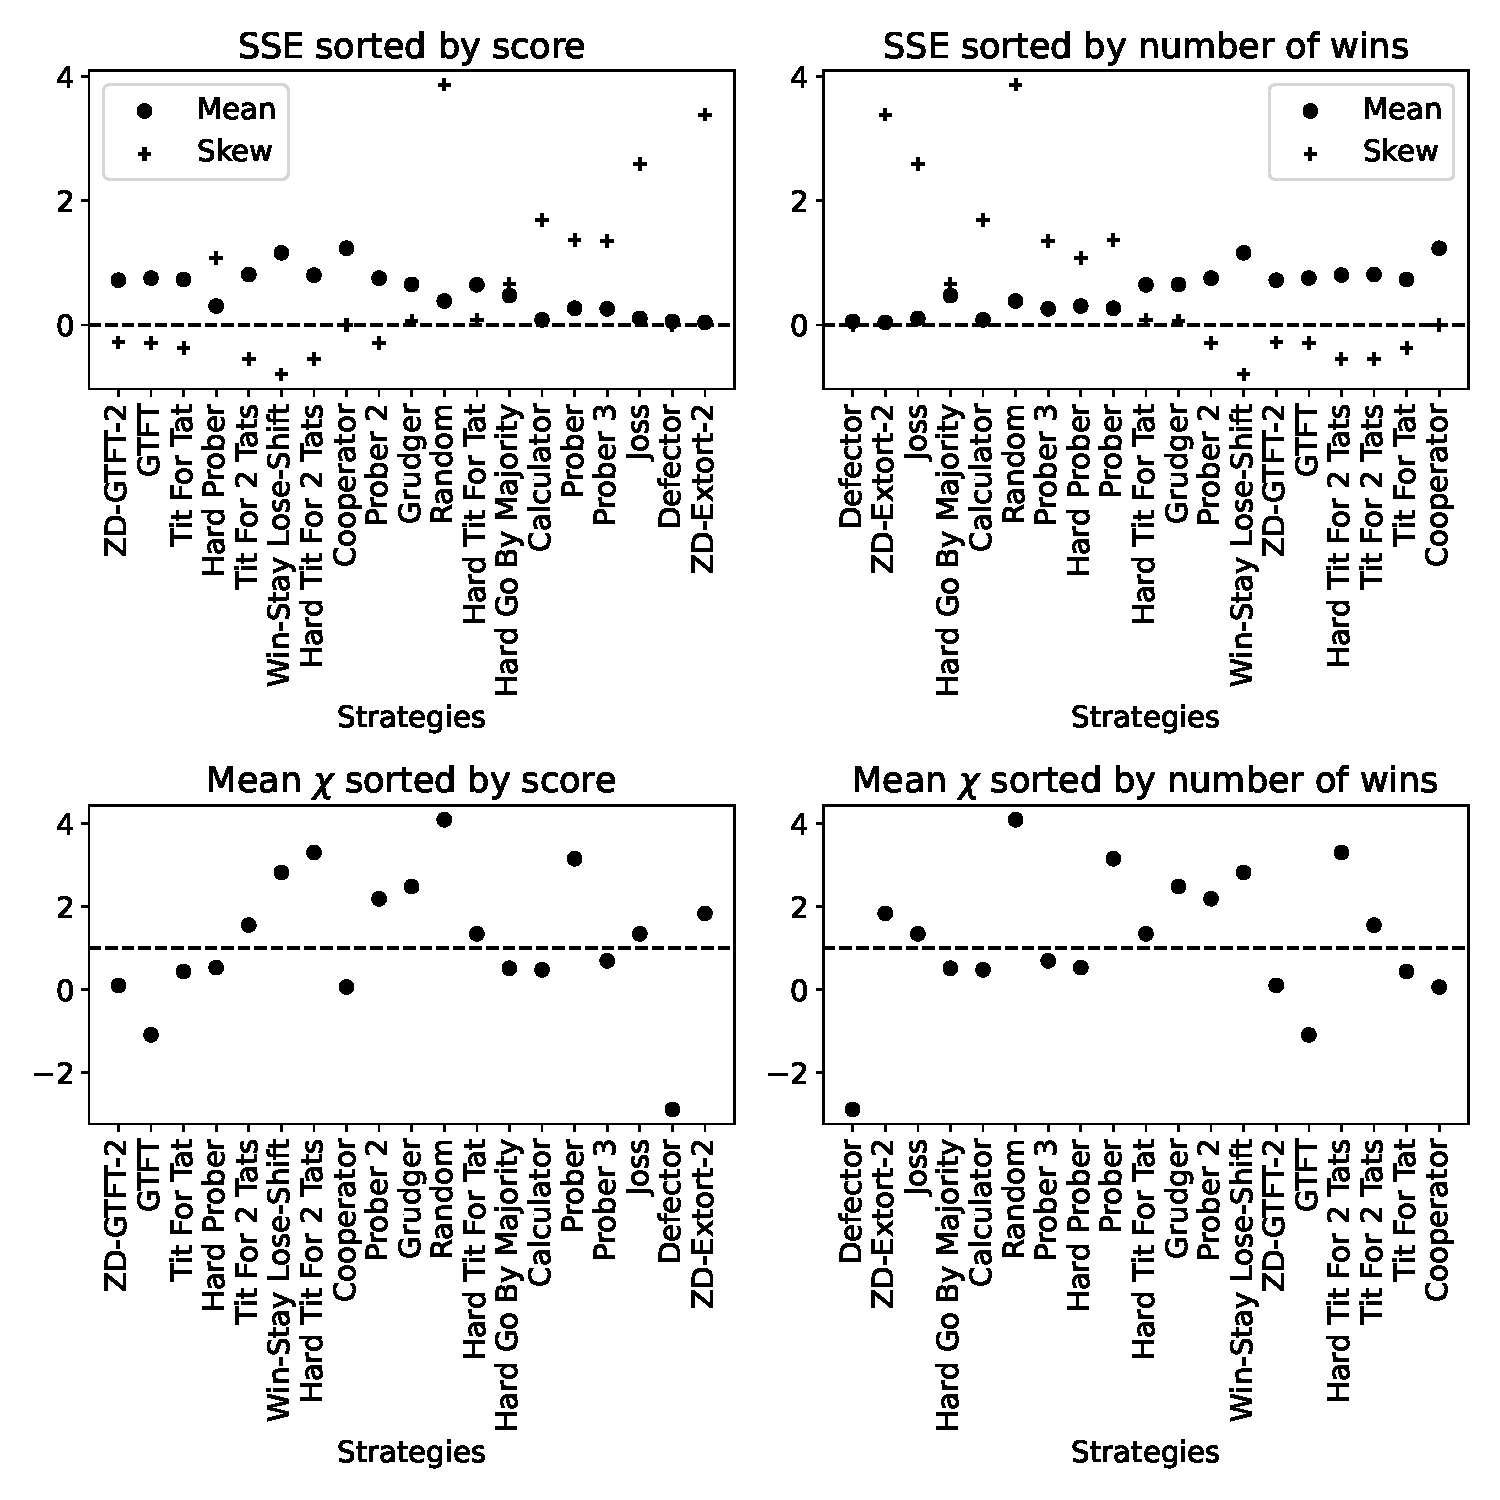
\includegraphics[width=.8\textwidth]{./assets/img/sserror_in_stewart_plotkin/main.pdf}
    \caption{\(\SSe\) and \(\chi\) for~\cite{Stewart2012},
        ordered both by number of wins and overall score. The dashed line shows
        the \(\chi=1\) boundary highlighting which strategies act in an
        extortionate manner. The strategies which a low variation in
        \(\SSe\) and high \(\chi\) win the most matches, although even the known
        extortionate strategy does not act in a perfectly extortionate manner in
        all matches. The strategies with a high score have a large variation in
        \(\SSe\).
        }
    \label{fig:sserror_in_stewart_plotkin}
\end{figure}

Here, the work of~\cite{Stewart2012} is extended by investigating a tournament
with 204strategies. The
results of this analysis are shown in
Figure~\ref{fig:sserror_and_probabilities_in_full}. The top ranking strategies
by number of wins act in an extortionate way (but not against all strategies) and
it can be seen that a small subgroup of strategies achieve mutual defection.
All the top ranking strategies according to score achieve mutual cooperation and
do not extort each other, however they \textbf{do} exhibit extortionate
behaviour towards a number of the lower ranking strategies.

\begin{figure}[!htbp]
    \centering
    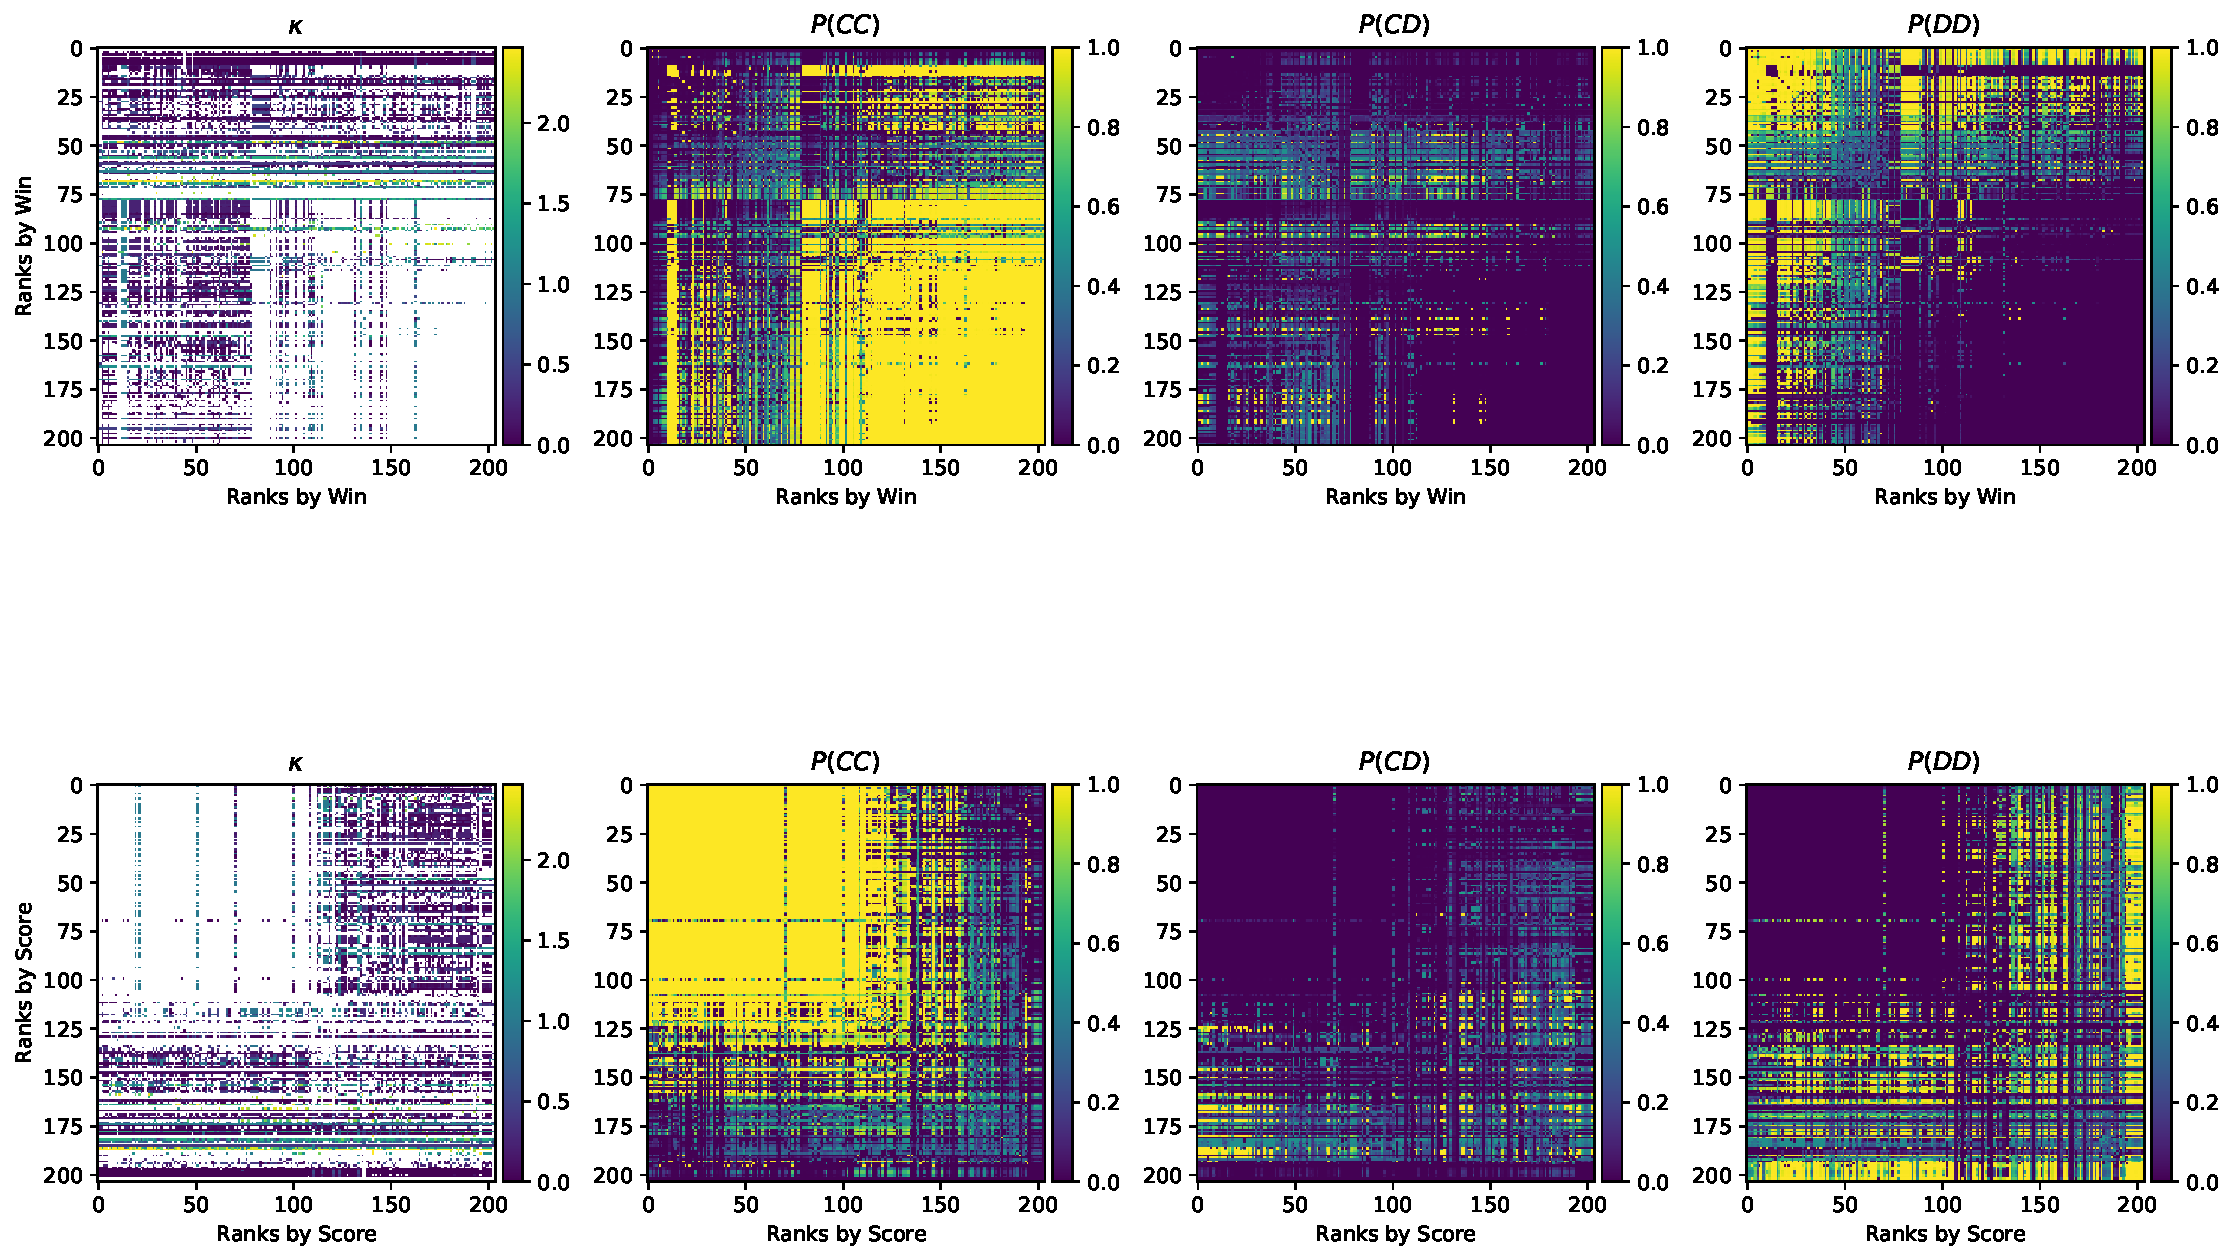
\includegraphics[width=.95\textwidth]{./assets/img/kappa_and_probabilities_in_full/main.pdf}
    \caption{\(\kappa\) for the strategies for the full
        tournament. For the \(\kappa\) plot only strategy
        interactions for which \(\chi>1\) are displayed. Note that
        \(P(DC)\) is not shown as it corresponds to the transpose of \(P(CD)\).}
    \label{fig:kappa_and_probabilities_in_full}
\end{figure}

A detailed look at selected strategies is given in
Table~\ref{tbl:overall_summary_results}. The high scoring strategies presented
have a large variation in \(\kappa\) whilst the ZD strategies have a low score
but high probability of winning. This evidences an idea proposed
in~\cite{adami2013evolutionary}: sophisticated strategies are able to recognise
their opponent and defend themselves against extortion.
The high ranking strategies were in fact trained to maximise
score~\cite{Harper2017} which seems to have created strategies able to extort
weaker strategies whilst cooperating with stronger ones. Indeed unconditional
extortion is self defeating.

\begin{table}[!hbtp]
    \begin{center}
    \tiny
    \begin{tabular}{rlrrrrrrrrrrr}
\toprule
 Rank &                   Name &  Score per turn &  $P($Win$)$ &  $P(CC)$ &  Overall $\kappa$ &  Min $\kappa$ &  5\% CI $\kappa$ &  Median $\kappa$ &  Mean $\kappa$ &  Std $\kappa$ &  95\% CI $\kappa$ &  Max $\kappa$ \\
\midrule
    1 &   EvolvedLookerUp2\_2\_2 &           2.944 &       0.230 &    0.673 &             0.230 &         0.015 &           0.059 &            1.235 &          1.087 &         0.482 &            1.721 &         2.471 \\
    2 &          Evolved HMM 5 &           2.944 &       0.205 &    0.718 &             0.102 &         0.030 &           0.086 &            1.235 &          0.808 &         0.540 &            1.235 &         1.235 \\
    3 &      PSO Gambler 2\_2\_2 &           2.913 &       0.204 &    0.624 &             0.200 &         0.005 &           0.059 &            1.235 &          0.911 &         0.539 &            1.236 &         2.471 \\
    4 &       PSO Gambler Mem1 &           2.908 &       0.211 &    0.715 &             0.068 &         0.054 &           0.066 &            1.235 &          0.720 &         0.575 &            1.235 &         1.235 \\
    5 &      PSO Gambler 1\_1\_1 &           2.906 &       0.221 &    0.696 &             0.138 &         0.022 &           0.055 &            1.235 &          0.749 &         0.543 &            1.235 &         1.235 \\
    7 &          Evolved ANN 5 &           2.893 &       0.225 &    0.682 &             0.001 &         0.000 &           0.001 &            1.235 &          0.814 &         0.572 &            1.235 &         1.235 \\
   31 &              ZD-GTFT-2 &           2.721 &       0.000 &    0.806 &             0.066 &         0.020 &           0.064 &            1.235 &          0.809 &         0.538 &            1.235 &         1.235 \\
   45 &               ZD-GEN-2 &           2.689 &       0.016 &    0.801 &             0.016 &         0.003 &           0.015 &            1.235 &          0.699 &         0.599 &            1.235 &         1.235 \\
   47 &              Eatherley &           2.682 &       0.000 &    0.828 &             0.084 &         0.000 &           0.003 &            1.235 &          0.904 &         0.479 &            1.235 &         1.235 \\
   69 &            Tit For Tat &           2.638 &       0.000 &    0.723 &             0.000 &         0.000 &           0.000 &            1.235 &          0.796 &         0.564 &            1.235 &         1.235 \\
   75 &                 Grumpy &           2.630 &       0.075 &    0.793 &             0.000 &         0.000 &           0.000 &            1.235 &          0.979 &         0.492 &            1.235 &         1.235 \\
   88 &    Win-Stay Lose-Shift &           2.616 &       0.099 &    0.649 &             1.235 &         1.000 &           1.000 &            1.235 &          1.206 &         0.077 &            1.235 &         1.235 \\
  103 &  Eventual Cycle Hunter &           2.565 &       0.067 &    0.770 &             0.000 &         0.000 &           0.003 &            1.235 &          0.753 &         0.584 &            1.235 &         1.235 \\
  107 &  Tricky Level Punisher &           2.537 &       0.062 &    0.828 &             0.000 &         0.000 &           0.000 &            1.235 &          0.711 &         0.595 &            1.235 &         1.235 \\
  127 &               Adaptive &           2.272 &       0.500 &    0.363 &             0.000 &         0.000 &           0.000 &            0.059 &          0.097 &         0.222 &            0.276 &         1.529 \\
  169 &                  Bully &           1.970 &       0.381 &    0.141 &             1.529 &         0.059 &           0.209 &            1.529 &          1.411 &         0.349 &            1.529 &         1.529 \\
  179 &             Alternator &           1.945 &       0.392 &    0.157 &             1.529 &         1.000 &           1.000 &            1.529 &          1.594 &         0.344 &            2.471 &         2.471 \\
  181 &               Negation &           1.941 &       0.356 &    0.141 &             1.529 &         0.292 &           1.229 &            1.529 &          1.486 &         0.207 &            1.529 &         2.005 \\
  183 &              Cycler DC &           1.931 &       0.324 &    0.149 &             1.529 &         0.529 &           0.529 &            1.529 &          1.274 &         0.419 &            1.529 &         1.529 \\
  188 &               Hopeless &           1.908 &       0.352 &    0.261 &             2.471 &         1.009 &           1.363 &            2.471 &          2.102 &         0.429 &            2.471 &         2.471 \\
  194 &         Gradual Killer &           1.892 &       0.354 &    0.439 &             0.000 &         0.000 &           0.000 &            0.089 &          0.148 &         0.187 &            0.298 &         1.235 \\
  196 &             Aggravater &           1.879 &       0.930 &    0.087 &             0.235 &         0.059 &           0.059 &            0.059 &          0.095 &         0.065 &            0.235 &         0.235 \\
  200 &            ZD-Extort-2 &           1.821 &       0.851 &    0.179 &             0.000 &         0.000 &           0.000 &            0.000 &          0.027 &         0.160 &            0.009 &         1.059 \\
  201 &            ZD-Extort-4 &           1.820 &       0.865 &    0.106 &             0.000 &         0.000 &           0.000 &            0.000 &          0.028 &         0.157 &            0.066 &         1.237 \\
  202 &             ZD-Extort3 &           1.810 &       0.862 &    0.133 &             0.000 &         0.000 &           0.000 &            0.000 &          0.027 &         0.161 &            0.014 &         1.060 \\
  203 &               Defector &           1.808 &       0.929 &    0.000 &             0.059 &         0.059 &           0.059 &            0.059 &          0.059 &         0.000 &            0.059 &         0.059 \\
  204 &              Handshake &           1.806 &       0.870 &    0.046 &             0.000 &         0.000 &           0.000 &            0.529 &          0.511 &         0.344 &            1.236 &         1.721 \\
\bottomrule
\end{tabular}

    \end{center}
    \caption{Summary of results for a selected list of strategies. The overall
             \(\kappa\) is computed by considering all transitions against all
             opponents.}
    \label{tbl:overall_summary_results}
\end{table}

\section{Evolutionary dynamics}\label{sec:evolutionary-dynamics}

From the large number of interactions a payoff matrix \(S\)
can be measured where \(S_{ij}\) denotes the score (using standard values of
\((R, S, T, P) = (3, 0, 5, 1)\)) of the \(i\)th strategy against the \(j\)th
strategy. Using this, the replicator equation describes the evolution of the
system based on a population density fitness function:

\begin{equation}\label{eqn:replicator_dynamics}
    \frac{dx_i}{dt} = x_i(S_i-x^TS x)
\end{equation}

Equation (\ref{eqn:replicator_dynamics}) is solved numerically through an
integration technique described in~\cite{Petzold1983} and
Figure~\ref{fig:replicator_dynamics} shows the evolution of the distribution of
the system: the various strategies are ranked by scores. It is clear to see that
only the high ranking strategies survive the evolutionary process (in fact,
only 39
have a final long run probability value greater than \(10 ^ {-2}\)).

\begin{figure}[!htbp]
    \centering
    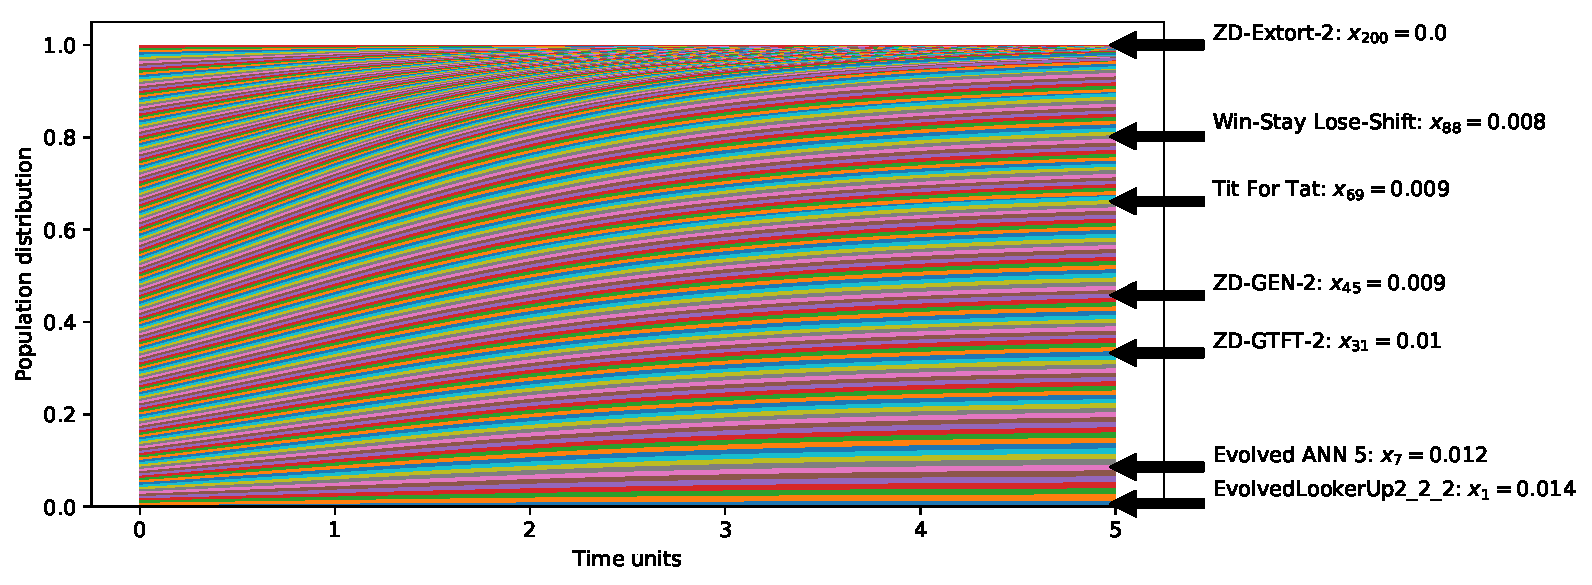
\includegraphics[width=.8\textwidth]{./assets/img/replicator_dynamics/main.pdf}
    \caption{Numerical simulation of the replicator equation
    (\ref{eqn:replicator_dynamics}): strategies are ordered by score. Some
    selected strategies are highlighted with their long run population
    distribution.}
    \label{fig:replicator_dynamics}
\end{figure}

In Figure~\ref{fig:compare-evolutionary-dynamics-to-kappa} linear models are
fitted to three summary measures of \(\kappa\) against the long run
probabilities \(s\) of (\ref{eqn:replicator_dynamics}). In all cases the
predictive power of these models is small (a low \(R^2\)) however, we note a
significant positive correlation between the standard deviation of \(\kappa\)
and \(s\). Indeed: strategies that perform strongly according to equation
(\ref{eqn:replicator_dynamics}) seem to be strategies that are able to modify
their memory one representation depending on the opponent.

\begin{figure}[!hbtp]
    \centering
    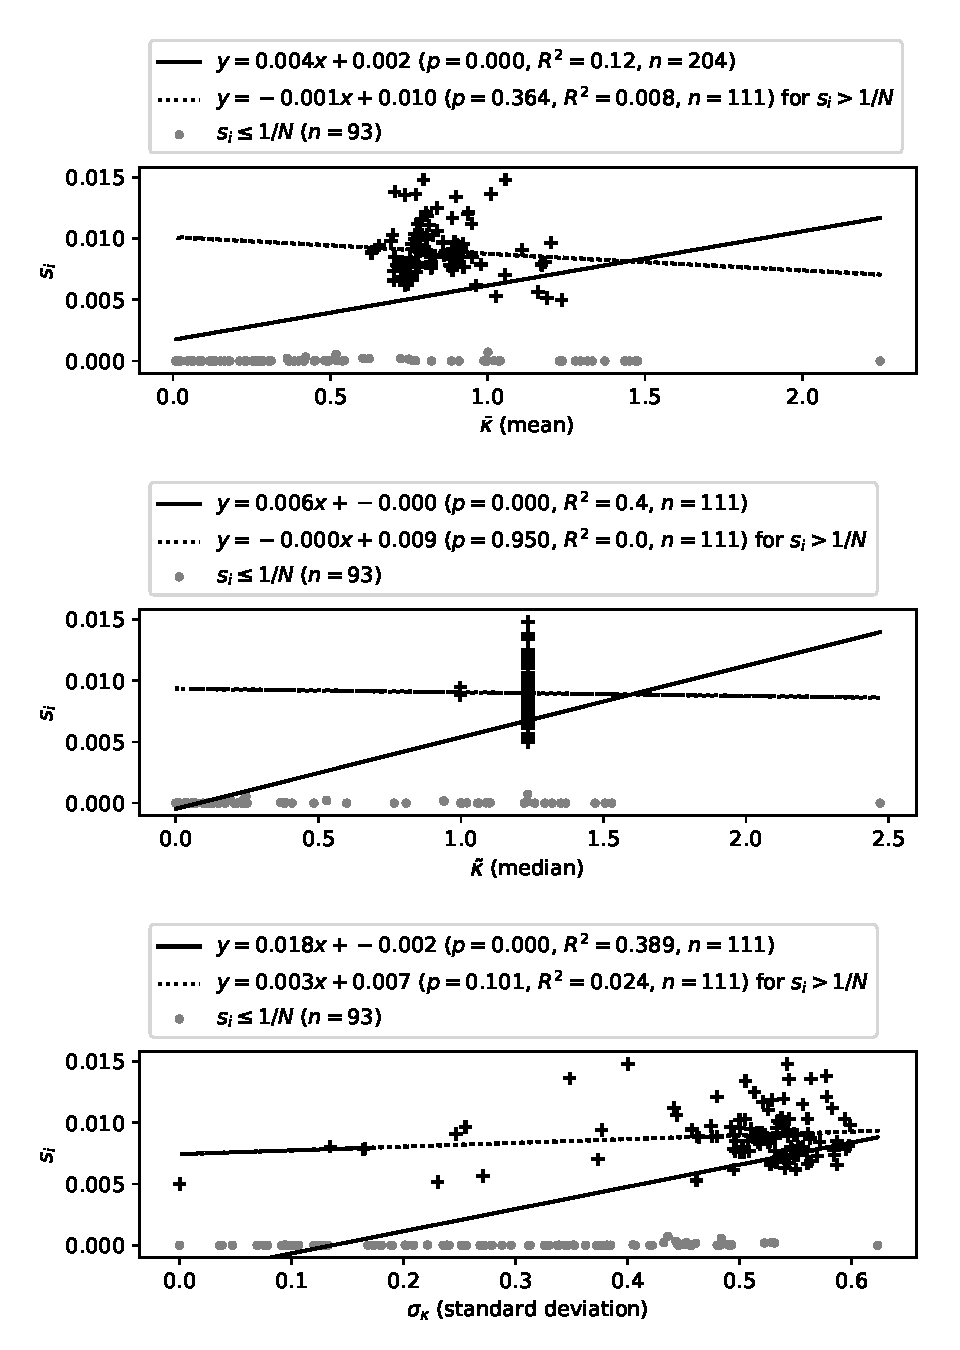
\includegraphics[width=\textwidth]{./assets/img/compare-evolutionary-dynamics-to-kappa/main.pdf}
    \caption{Linear regression analysis of long run probabilities of
    (\ref{eqn:replicator_dynamics}) against the mean, median and standard
    deviation of \(\kappa\) (for a given strategy).}
    \label{fig:compare-evolutionary-dynamics-to-kappa}
\end{figure}

In~\cite{Moran1707} a large data set of pairwise fixation probabilities in the
Moran process is made available at~\cite{vincent_knight_2017_1040129}
Figure~\ref{fig:compare-fixation-to-kappa} shows linear models fitted to three
summary measures of \(\kappa\) and the mean (over population size \(N\) and
opponents) value of \(x_1\cdot N\). This specific measure of fixation is chosen
as \(x_1\) is usually compared to the neutral fixation probability of \(1 / N\).
As was noted in~\cite{Moran1707}, the specific case of \(N=2\) differs from all
other population sizes which is why it is presented in isolation. Similarly to
the conclusions from Figure~\ref{fig:compare-evolutionary-dynamics-to-kappa}
we note that there is a significant relationship between the variability of
\(\kappa\) and the ability for a strategy to become fixed.

\begin{figure}[!hbtp]
    \centering
    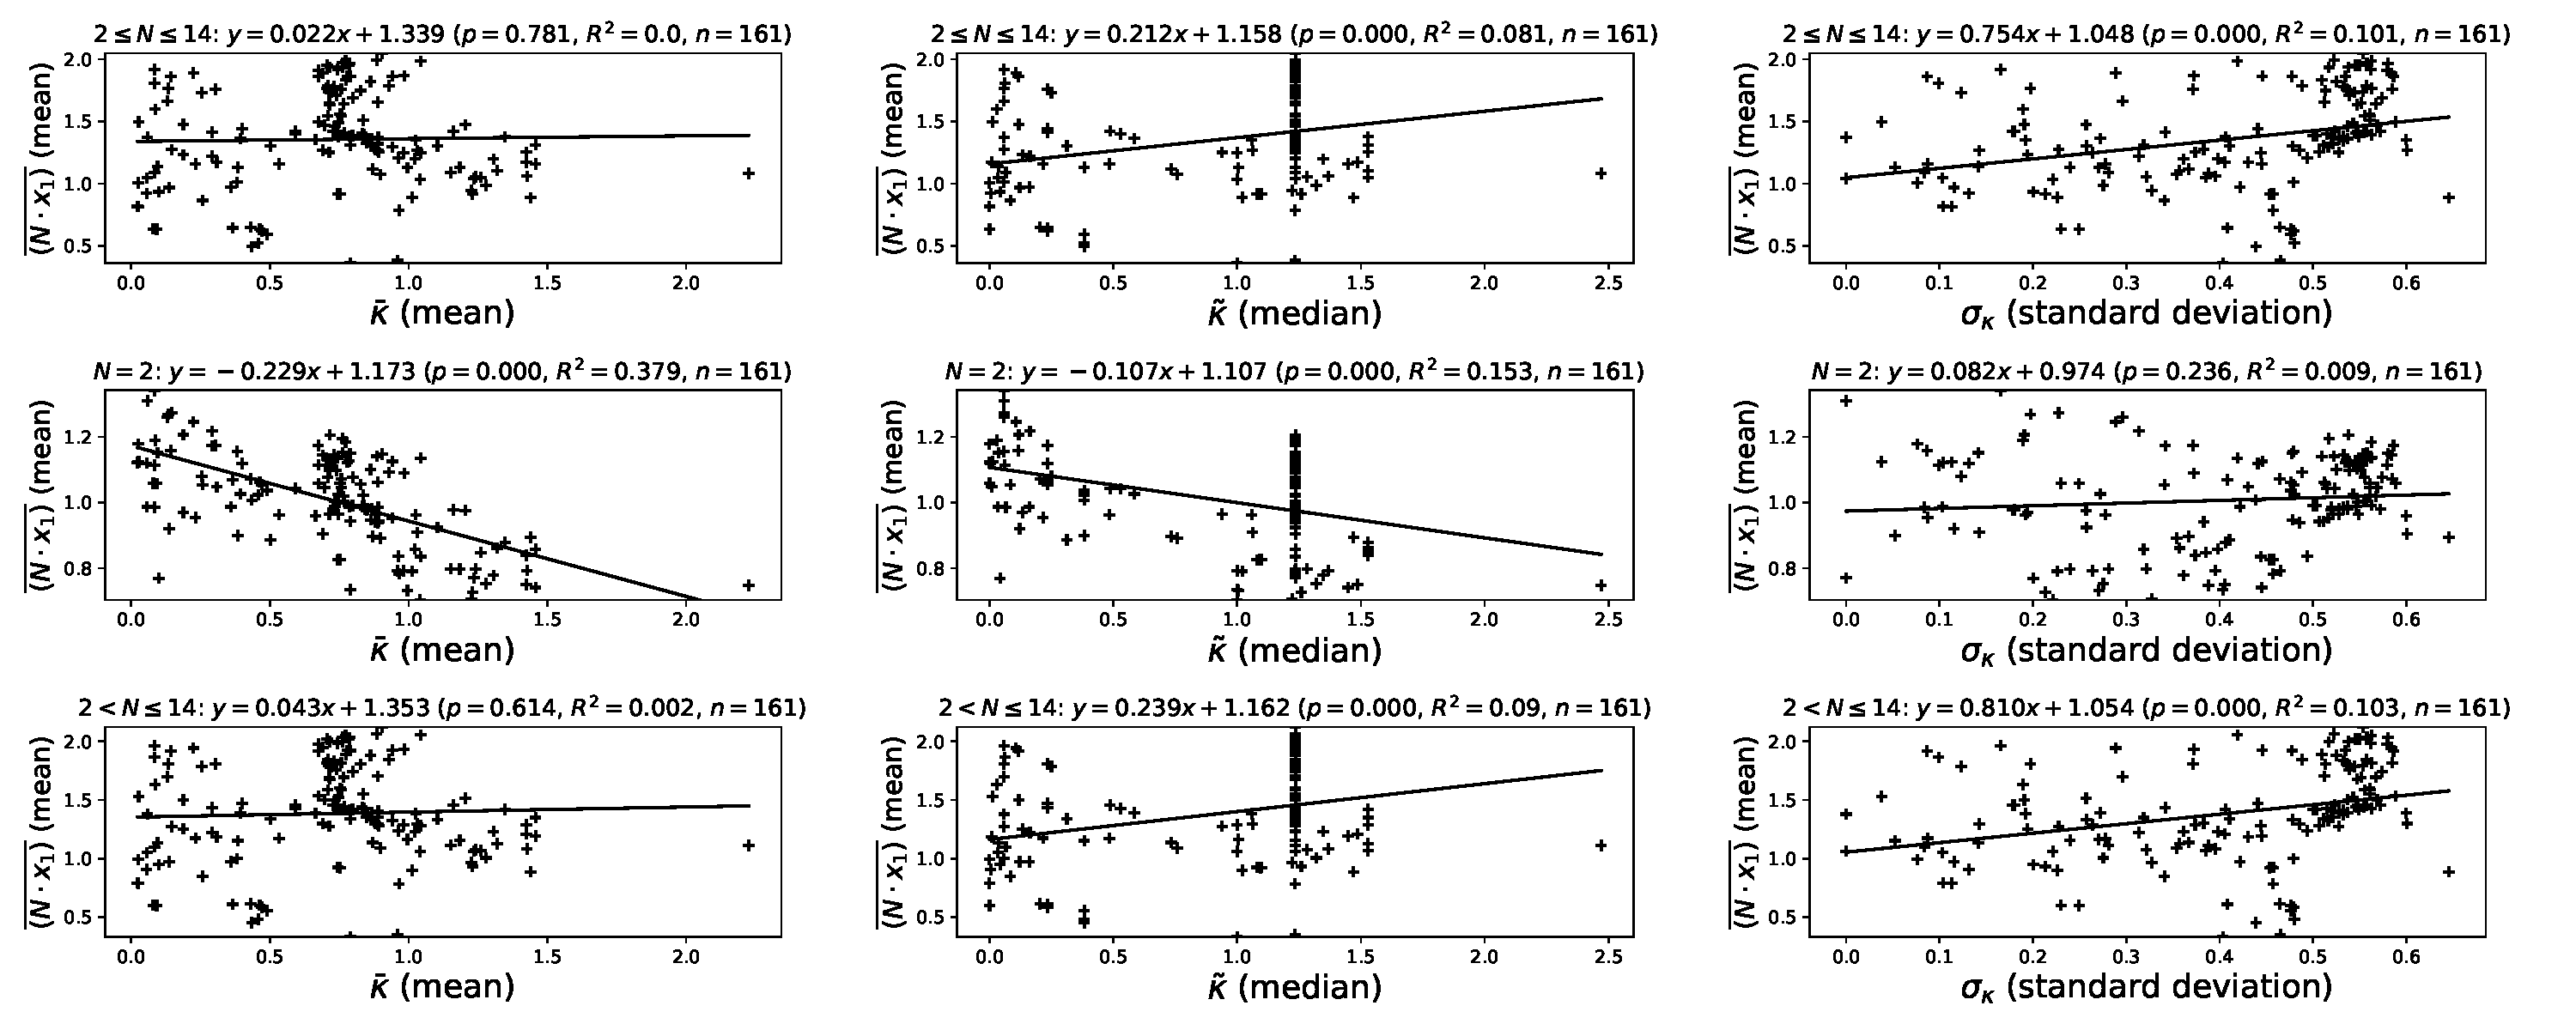
\includegraphics[width=\textwidth]{./assets/img/compare-fixation-to-kappa/main.pdf}
    \caption{Linear regression analysis of pairwise fixation probabilities
    from~\cite{Moran1707} against the mean, median and standard deviation of
    \(\kappa\) (for a given strategy).}
    \label{fig:compare-fixation-to-kappa}
\end{figure}

Note that in both Figures~\ref{fig:compare-evolutionary-dynamics-to-kappa}
and~\ref{fig:compare-fixation-to-kappa}, there is a large proportion of
strategies with \(\tilde\kappa\approx1.23\). This corresponds to \(p=(1,1,1,1)\)
(a cooperator) and indicates cooperative behaviour.

These findings confirm the work of~\cite{Moran1707} in which sophisticated
strategies resist evolutionary invasion of shorter memory strategies. This also
confirms the work of~\cite{adami2013evolutionary, hilbe2015partners} which
proved that ZD strategies where not evolutionarily stable due to the fact that
they score poorly against themselves.

The work also provides strong evidence to the importance of adaptability:
strategies that offer a variety of behaviours corresponding to a higher standard
deviation of \(\kappa\) are significantly more likely to survive the
evolutionary process. This corresponds to the following quote
of~\cite{darwin1869origin}:

\begin{quote}
``It is not the most intellectual of the species that survives; it is not the
strongest that survives; but the species that survives is the one that is able
to adapt to and to adjust best to the changing environment in which it finds
itself.''
\end{quote}

\section{Conclusion}\label{sec:conclusion}

This work defines an approach to measure whether or not a player is playing a
strategy that corresponds to an extortionate strategy as defined
in~\cite{Press2012}: a mathematical model for suspicion. All extortionate
strategies have been classified as lying on a triangular plane.  This rigorous
classification fails to be robust to small measurement error, thus a statistical
approach is proposed approximating the solution of a linear system. Using this,
a large number of pairwise interactions is simulated.

The work of~\cite{Press2012}, whilst showing that a clever approach to taking
advantage of another memory-one strategy exists: this is not the full story.
Though the elegance of this result is very attractive, just as the simplicity of
the victory of Tit For Tat in Axelrod's original tournaments was, it is
incomplete.  Extortionate strategies achieve a high number of wins but they do
not achieve a high score and fail to be evolutionarily stable.

Instead, it is in fact the more sophisticated strategies that are able to adapt
to their opponent and act extortionately against weaker strategies and
cooperate with like minded strategies that perform well.

Following Axelrod's seminal work~\cite{Axelrod1980, Axelrod1980a}, it was
commonly thought that evolutionary cooperation required strategies that followed
a simple set of rules. The discovery/definition of extortionate
strategies~\cite{Press2012} seemingly showed that complex strategies could be
taken advantage of. In this manuscript it has been shown that not only is it
possible to detect and prevent extortionate behaviour but that more complex
strategies can be evolutionary stable. The complex strategies in question were
obtained through reinforcement learning approaches~\cite{Harper2017, Moran1707}.
This work demonstrates the possibility for the evolution of cooperation
through suspicion.

\section*{Acknowledgements}

The following open source software libraries were used in this research:

\begin{itemize}
    \item The Axelrod ~\cite{Knight2016, Knight2018} library (IPD strategies and
        tournaments).
    \item The sympy library~\cite{Meurer2017} (verification of all symbolic
        calculations).
    \item The matplotlib~\cite{Droettboom2018} library (visualisation).
    \item The pandas~\cite{Structures2010}, dask~\cite{Dask2016} and
        NumPy~\cite{Oliphant2015} libraries (data manipulation).
    \item The SciPy~\cite{Jones2001} library (numerical integration of the
        replicator equation).
\end{itemize}

This work was performed using the computational facilities of the Advanced
Research Computing @ Cardiff (ARCCA) Division, Cardiff University.

\printbibliography

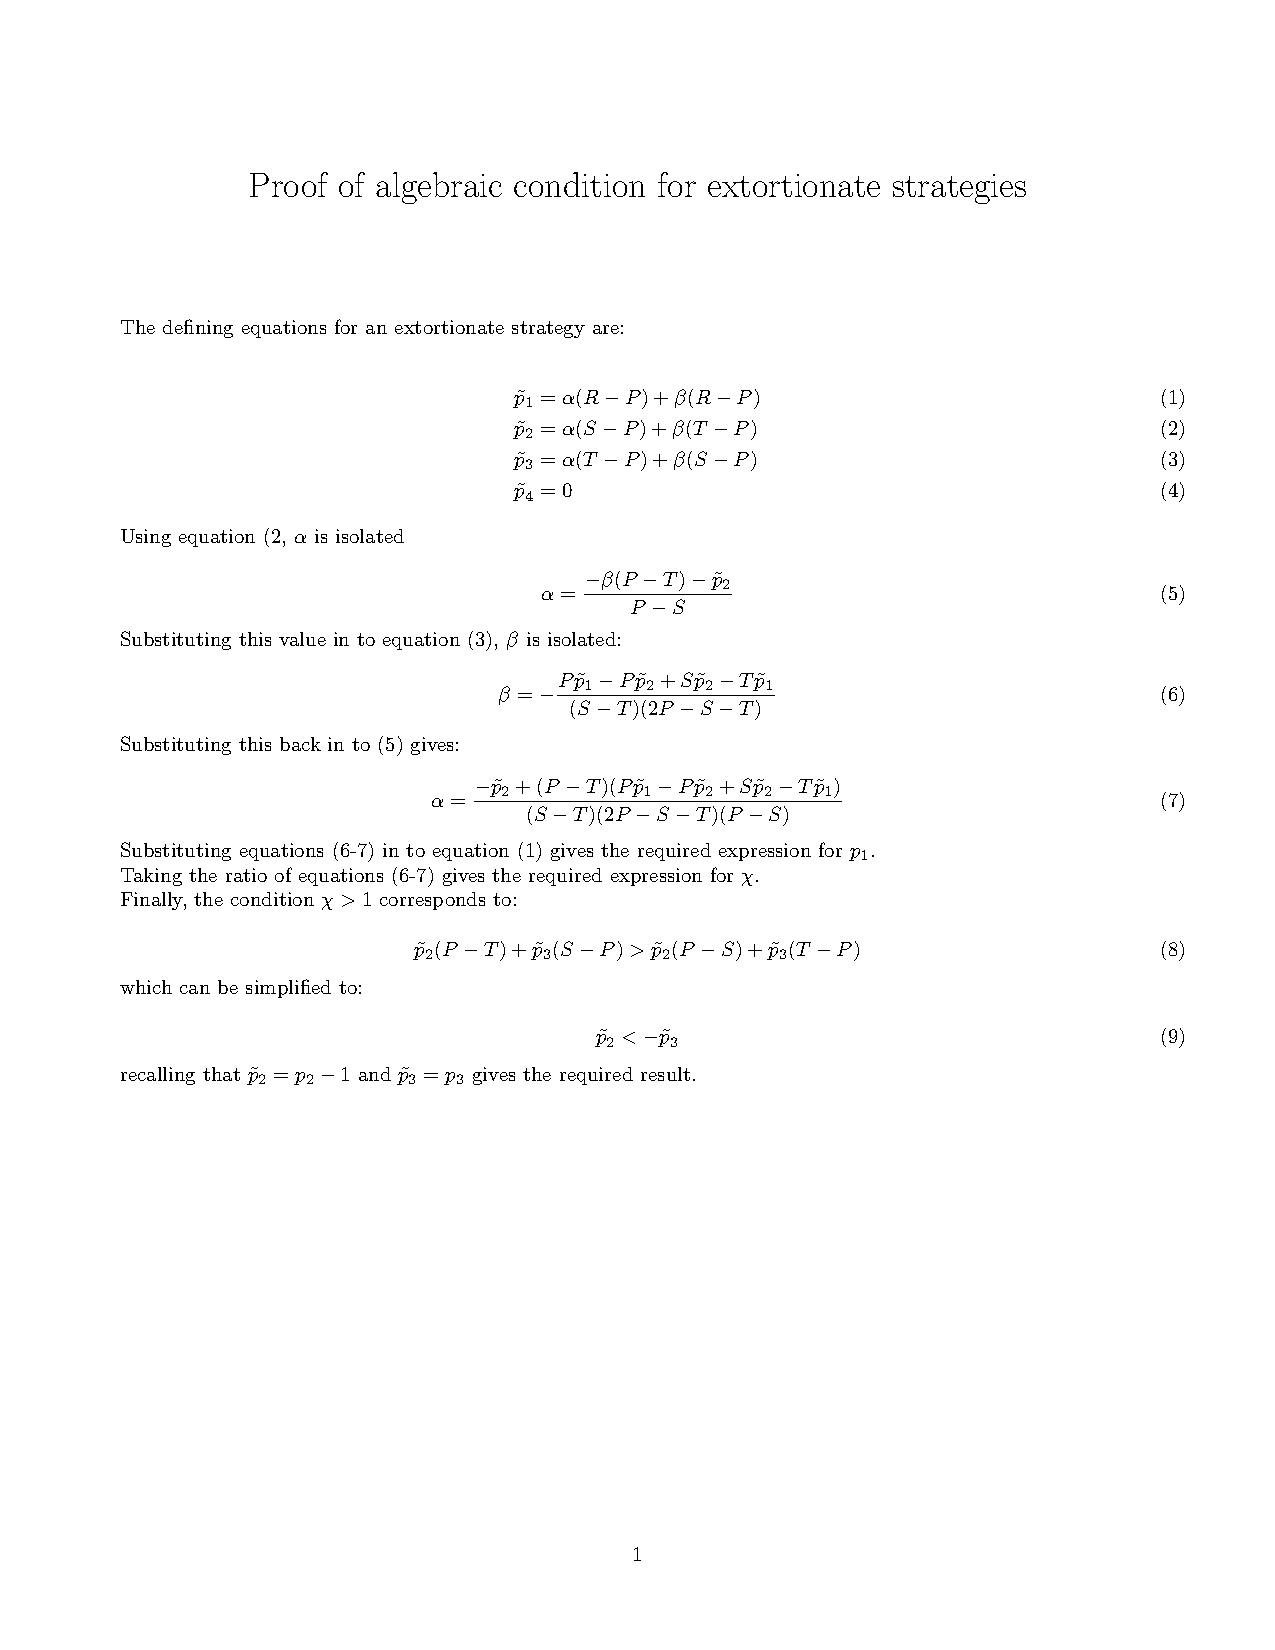
\includepdf{assets/pdf/proof_of_form_of_extortionate_strategies/main.pdf}
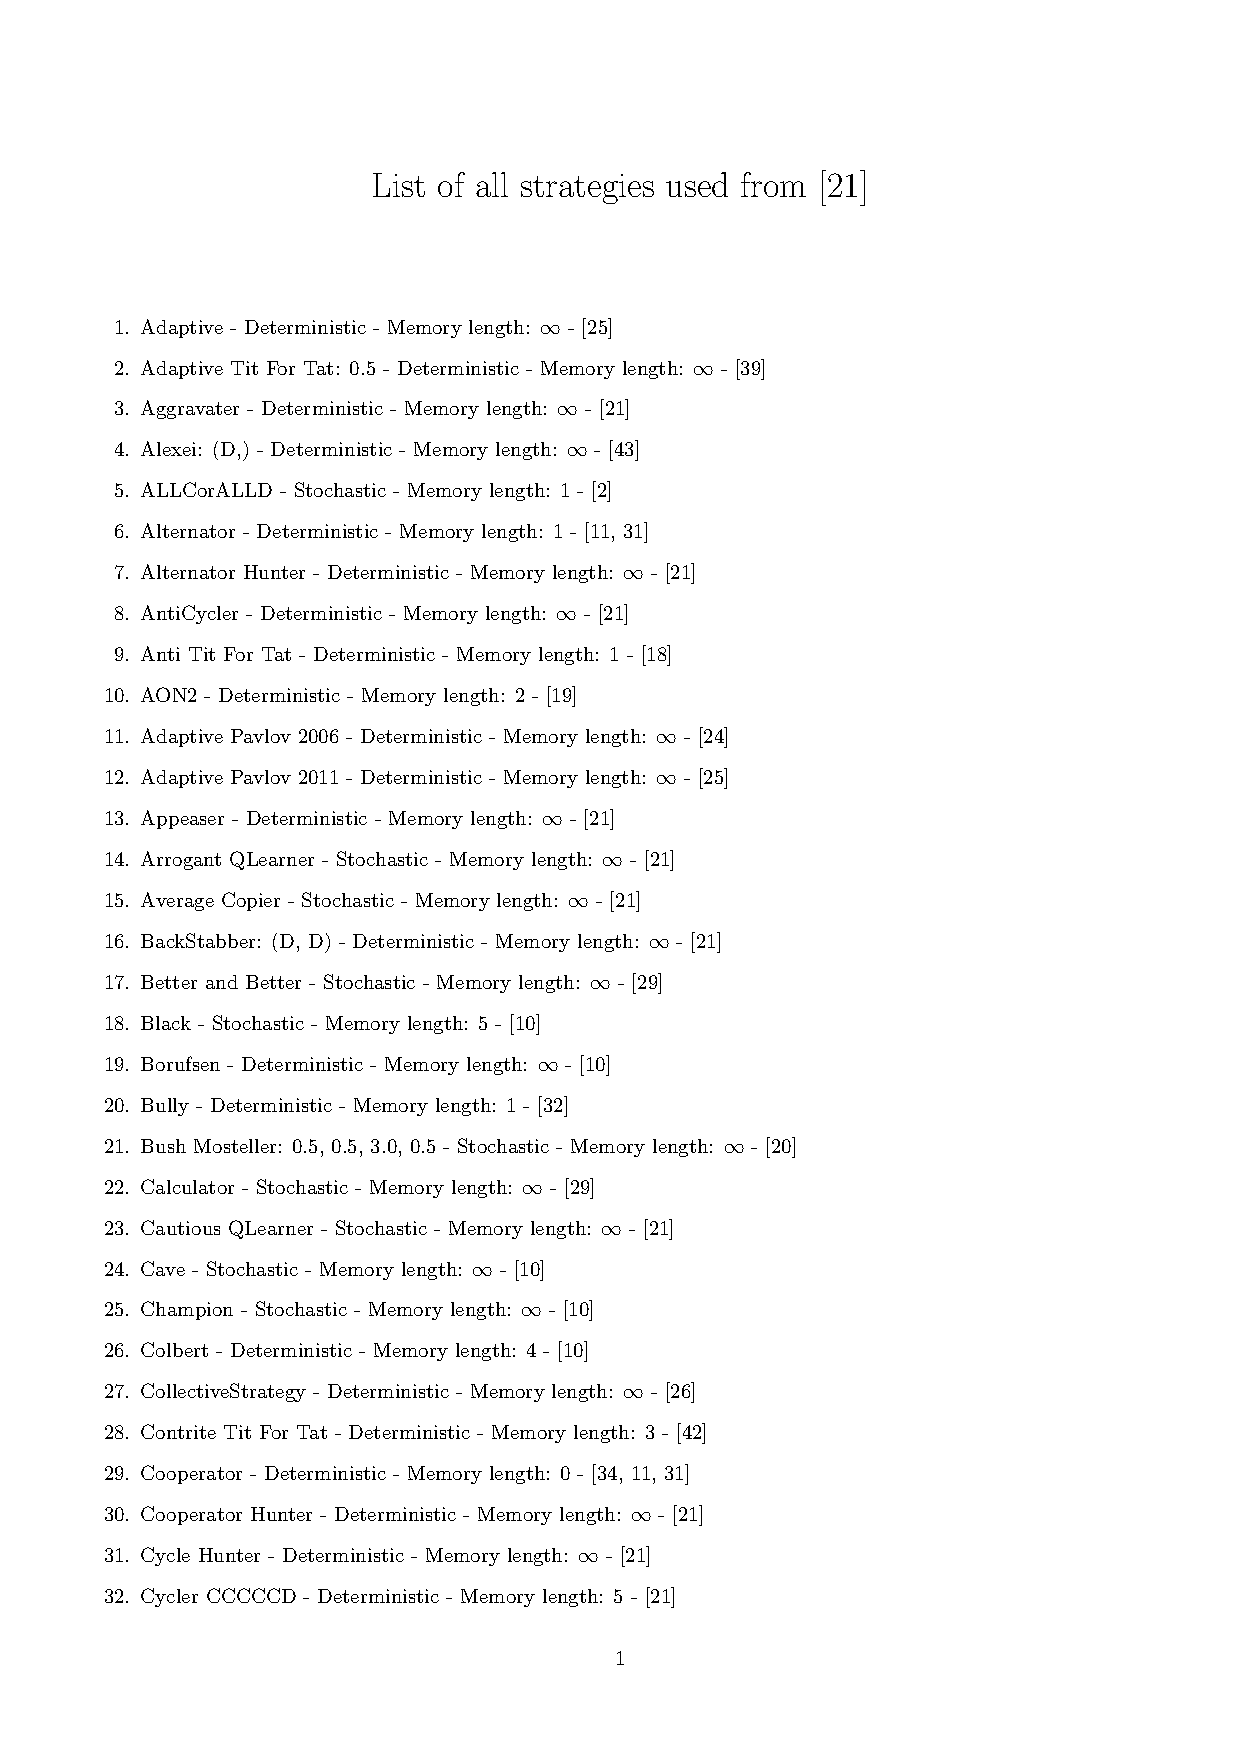
\includepdf[pages={1-}]{assets/pdf/list_of_strategies/main.pdf}

\end{document}
